%%%%%%%%%%%%%%%%%%%%%%%%%%%%%%%%%%%%%%%%%%%%%%%%%%%%%%%%%%%
\section{Theory}
\label{sec:theory}
%%%%%%%%%%%%%%%%%%%%%%%%%%%%%%%%%%%%%%%%%%%%%%%%%%%%%%%%%%%
\begin{figure*}[!htb]
\begin{center}
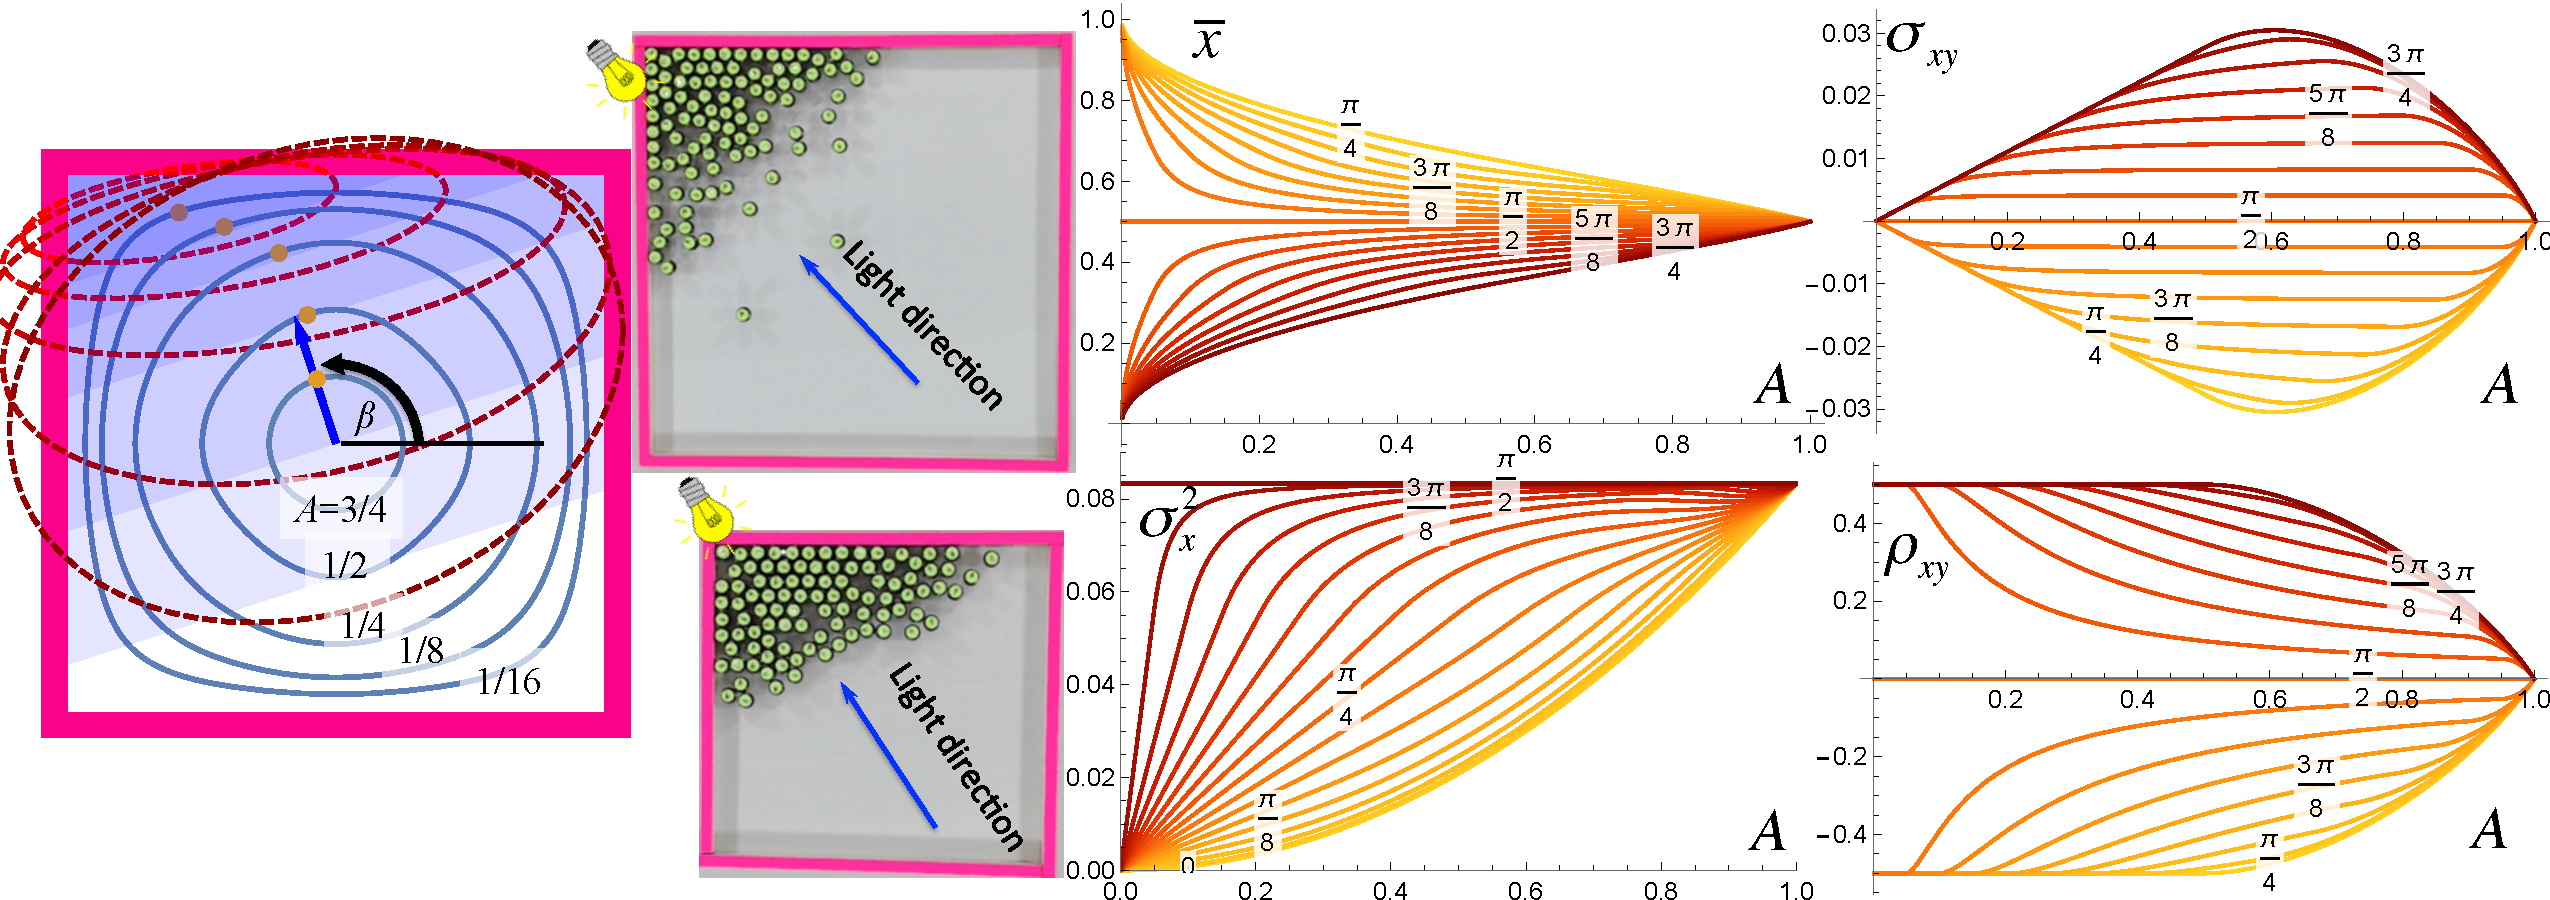
\includegraphics[width=\linewidth]{SquareFill.pdf} 
\vspace{-1em}
\caption{Pushing the swarm against a square boundary wall allows limited control of the shape of the swarm, as a function of swarm area $A$ and the commanded movement direction $\beta$. Left plot shows locus of possible mean positions for five values of $A$.  The locus morphs from a square to a circle as $A$ increases.  The covariance ellipse for each $A$ is shown with a dashed line. Center shows two corresponding arrangements of kilobots.  At right is $\bar{x}(A), \sigma_{xy}(A), \sigma_x^2(A),$ and $\rho(A)$ for a range of $\beta$ values. See online interactive demonstration at \citep{Zhao2016mathematicaSquare}.}
\label{fig:SquareFill}
\end{center}
\end{figure*} 
\begin{figure*}[!htb]
\begin{center}
\vspace{-1em}
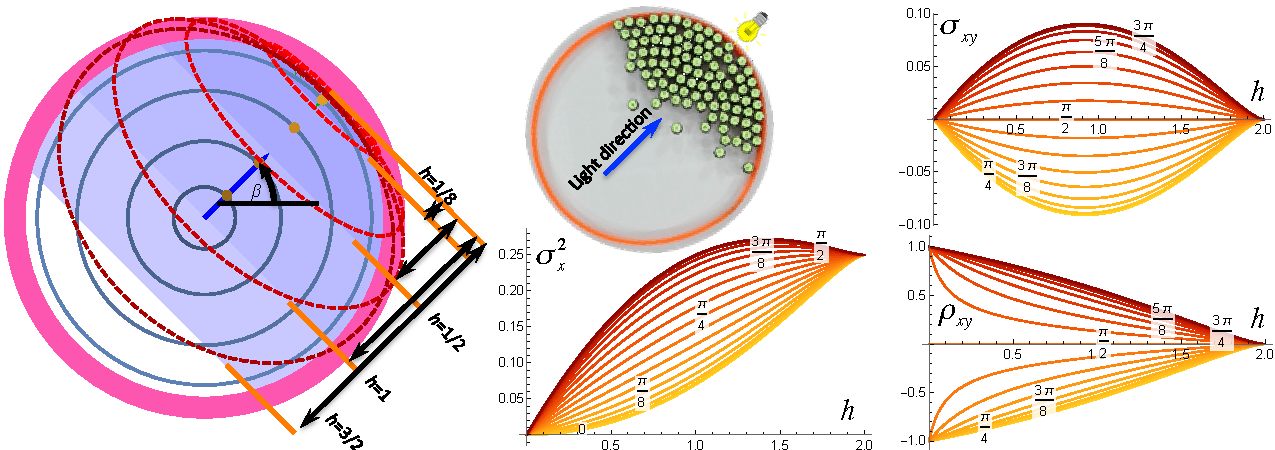
\includegraphics[width=\linewidth]{CircleFill.pdf} 
\vspace{-1em}
\caption{Pushing the swarm against a circular boundary wall allows limited control of the shape of the swarm, as a function of the fill level $h$ and the commanded movement direction $\beta$. Left plot shows locus of possible mean positions for four values of $h$. The locus of possible mean positions are concentric circles. See online interactive demonstration at \citep{Zhao2016mathematica}.}  
\label{fig:CircleFill}
\end{center}
\end{figure*} 

\subsection{Using Boundaries: stable configurations of a swarm}\label{subsec:FluidInTank}
One method to control a swarm's shape in a bounded workspace is to simply push in a given direction until the swarm conforms to the boundary.
\paragraph{Square workplace}
%The formulas for means $(\bar{x},\bar{y})$, covariance $(\sigma^2_x,\sigma^2_y,\sigma_{xy})$, and correlation $\rho_{xy}$ are as follows: 
We first examine the mean $(\bar{x},\bar{y})$, covariance $(\sigma^2_x,\sigma^2_y,\sigma_{xy})$, and correlation $\rho_{xy}$ of a very large swarm of robots as they move inside a square workplace under the influence of gravity pointing in the direction $\beta$. The swarm is large, but the robots are small in comparison, and together occupy a constant area $A$ ranging from [0,1]. Under a global input such as gravity, they flow like water, moving to a side of the workplace and forming a polygonal shape, as shown in Fig.~\ref{fig:SquareFill},  see also \citep{Zhao2016mathematicaSquare}.

The range for the global input angle $\beta $ is [0,2$\pi $). In this range, the swarm assumes eight different polygonal shapes. 
These shapes alternate between triangles and trapezoids when the area $A$$<$1/2, and between squares with one corner removed and trapezoids when $A$$>$1/2.

Computing means, variances, covariance, and correlation requires integrating over the region $R$, the region containing the swarm:  %This is simplified using an indicator function $\bm{1}_A(x,y)$ that returns 1 if inside the region containing the swarm, and 0 else. 
%The formulas for means $(\bar{x},\bar{y})$, covariance $(\sigma^2_x,\sigma^2_y,\sigma_{xy})$, and correlation $\rho_{xy}$ are as follows: %, integrated over the unit square with $x$ and $y$ from 0 to 1:

\begin{align}
\bar{x} &=\frac{\iint_R x \,dx\,dy}{A} \label{eq:meanInSquareWorkspace}
\text{, }\qquad \bar{y}=\frac{\iint_R y \,dx\,dy}{A} \\
%\end{align}
%\begin{align}
\sigma^2_x &=\frac{\iint_R \left(x-\bar{x}\right)^2  \,dx \,dy}{A}  \label{eq:varInSquareWorkspace}
\text{, } \sigma^2_y =\frac{\iint_R  \left(y-\bar{y}\right)^2 \,dx \,dy}{A}\\
%\end{align}
%\begin{align}
\sigma_{xy} &= \frac{\iint_R  \left(x-\bar{x}\right) \left(y-\bar{y}\right) \, dx \,dy}{A} \label{eq:covAndcorrInSquareWorkspace}
\text{, }\rho_{xy} = \frac{\sigma^2_x}{\sigma_x\sigma_y}
\end{align}

The region of integration $R$ is the polygon containing the swarm. If $A<1/2$ and the force angle is $\beta$, the mean when $R$ is a triangular region in the lower-left corner is:
\begin{align}\label{eq:meanInSquareWorkspaceLL}
\bar{x}(A,\beta) &= \frac{\int_0^{\sqrt{2 A \tan (\beta)}} \left(\int_0^{\cot (\beta) \left(\sqrt{2 A \tan (\beta)}-x\right)} x \, dy\right) \, dx}{A} \nonumber \\
	&=\frac{ \sqrt{2}}{3} \sqrt{A \tan (\beta )}\\
\bar{y}(A,\beta) &= \frac{\int_0^{\sqrt{2 A \tan (\beta)}} \left(\int_0^{\cot (\beta) \left(\sqrt{2 A \tan (\beta)}-x\right)} y \, dy\right) \, dx}{A} \nonumber\\
	&=\frac{\sqrt{2}}{3}  \sqrt{A \cot (\beta )}
\end{align}
The full equations are included in the appendix~\citep{2016arXiv160901830S}, and are summarized in Fig.~\ref{fig:SquareFill}. A few highlights are that the correlation is maximized $\pm$1/2 when the swarm is in a triangular shape. The covariance of a triangle is always $\pm(A/18)$. Variance is minimized in the direction of $\beta$ and maximized orthogonal to $\beta$ when the swarm is in a rectangular shape. The range of mean positions are maximized when $A$ is small.

%%%%%%%%%%%%%%%%%%%%%%%%%%%%%%%
\paragraph{Circular workplace}
Though rectangular boundaries are common in artificial workspaces, biological workspaces are usually rounded.
Similar calculations can be made for a circular workspace.  The workspace is a circle centered at (0,0) with radius 1 and thus area $\pi$.
For notational simplicity, the swarm is parameterized by the global control input signal $\beta$ and the fill-level $h$.  
Under a global input, the robot swarm fills the region under a chord with area
\begin{align}
A(h) = \arccos(1-h)-(1-h) \sqrt{(2-h) h}.
\end{align}
For a circular workspace, the locus of mean positions are aligned with $\beta$ and the mean position is at radius $r(h)$ from the center:
\begin{align}
r(h) = \frac{2 (-(h-2) h)^{3/2}}{3 \left(\sqrt{-(h-2) h} (h-1)+\arccos(1-h)\right)}
\end{align}
Variance $\sigma^2_x(\beta,h)$ is maximized at $\beta = \pi/2+n \pi$ and $h\approx1.43$, while covariance is maximized at $\beta = \pi3/4+n \pi$ and $h\approx0.92.$ For small $h$ values, correlation approaches $\pm1$. Results are displayed in Fig.~\ref{fig:CircleFill}, see also \citep{Zhao2016mathematica}.

%Smashing the swarm to the corner walls will cause some correlation between \emph{x} and \emph{y} axes. Eq. ~\ref{eq:Wall} shows the relation between number of robots and area provided and the correlation we can reach with it.
%%TODO: ADD the equation for showing the correlation Vs area, vs number of robots
% This equation shows that we are not able to reach high correlations bigger than $|0.5|$. Fig. ~\ref{fig:wallCorrelation} shows the different mean positions and correlations we are able to reach. There are ways and corridors that the swarm needs to pass and also to keep the majority of it. If we use the wall corners technique and the way needs a very high correlation to pass, a remarkable number of the swarm members will be lost, and we may lose track of them due to their small size. Meanwhile, the variance of the swarm would get bigger and bigger that it would not anymore be able to deliver sufficient payloads. For this reason we have thought another idea which uses \emph{friction} to make correlations.
%


\subsection{Using Boundaries: Friction and Boundary Layers}\label{subsec:WallFriction}
Global inputs move a swarm uniformly.  
Shape control requires breaking this uniform symmetry.  
A swarm inside an axis-aligned rectangular workspace can reduce variance normal to a wall by simply pushing the swarm into the boundary. 
Controlling covariance by pushing the swarm into a boundary requires changes to the boundary.  
An obstacle in the lower-right corner is enough to generate positive covariance, but generating both positive and negative covariance requires additional obstacles.  
Requiring a special obstacle configuration also makes shape control dependent on the local environment. 
Instead of pushing our robots directly into a wall, this paper examines an oblique approach, by using boundaries that generate friction with the robots.  These frictional forces are  sufficient to break the symmetry caused by uniform inputs.  Robots touching a wall have a friction force that opposes movement along the boundary.  
This causes robots along the boundary to move more slowly than robots in free-space. 
  
Let the control input be a vector force $\vec{F}$ with magnitude $F$ and orientation $\theta$ with respect to a line perpendicular to and into the nearest boundary. $N$ is the normal or perpendicular force between the robot and the boundary. The force of friction $F_f$ is nonzero if the robot is in contact with the boundary and  $|\theta| < \pi/2$. The resulting net force on the robot, $F_{\text{\emph{forward}}}$, is aligned with the wall and given by
\begin{align}
F_{\text{\emph{forward}}} &=  F \sin(\theta) - F_f  \nonumber \\
\text{where }  F_f &= \begin{cases}  \mu_f N, &  \mu_f N < F \sin(\theta)  \label{eq:frictionmodel}  \\
F \sin(\theta), & \text{else} \end{cases} \\ %\sign(F \sin(\theta) ) \cdot  \max(0, | F sin\theta |- |F_f|)
\text{and } N &= F \cos(\theta) \nonumber
\end{align}
 Fig.~\ref{fig:friction} shows the resultant forces on two robots when one is touching a wall. 
Though each receives the same inputs,  they experience different net forces.
  For ease of analysis, the following algorithms assume $\mu_f$ is infinite and robots touching the wall are prevented from sliding along the wall.
This means that if one robot is touching the wall and another robot is free, the touching robot will not move when the control input is parallel or into the wall. 
There are many alternate models of friction that also break control symmetry. Fig.~\ref{fig:friction}c shows fluid flow along a boundary.  Fluid in the free-flow region moves uniformly, but flow decreases to zero in the boundary layer.  
\begin{align}
%u(y) = u_0 \left(1- \frac{(y-h)^2}{h^2}\right) = u_0 \frac{y}{h} \left(2- \frac{y}{h}\right) \label{eq:boundarylayerflow} THiS EQUATION IS TERRIBLE! PLOT IT.
F_{forward}(y) &= F - F_f\begin{cases}  \left( \frac{y-h}{h} \right)^2  , &  y<h \label{eq:boundarylayerflow} \\
0, & \text{else} \end{cases}
\end{align}

The next section shows how a system with friction model \eqref{eq:frictionmodel} and two orthogonal walls can arbitrarily position two robots. 
\begin{figure}[h]
\begin{center}
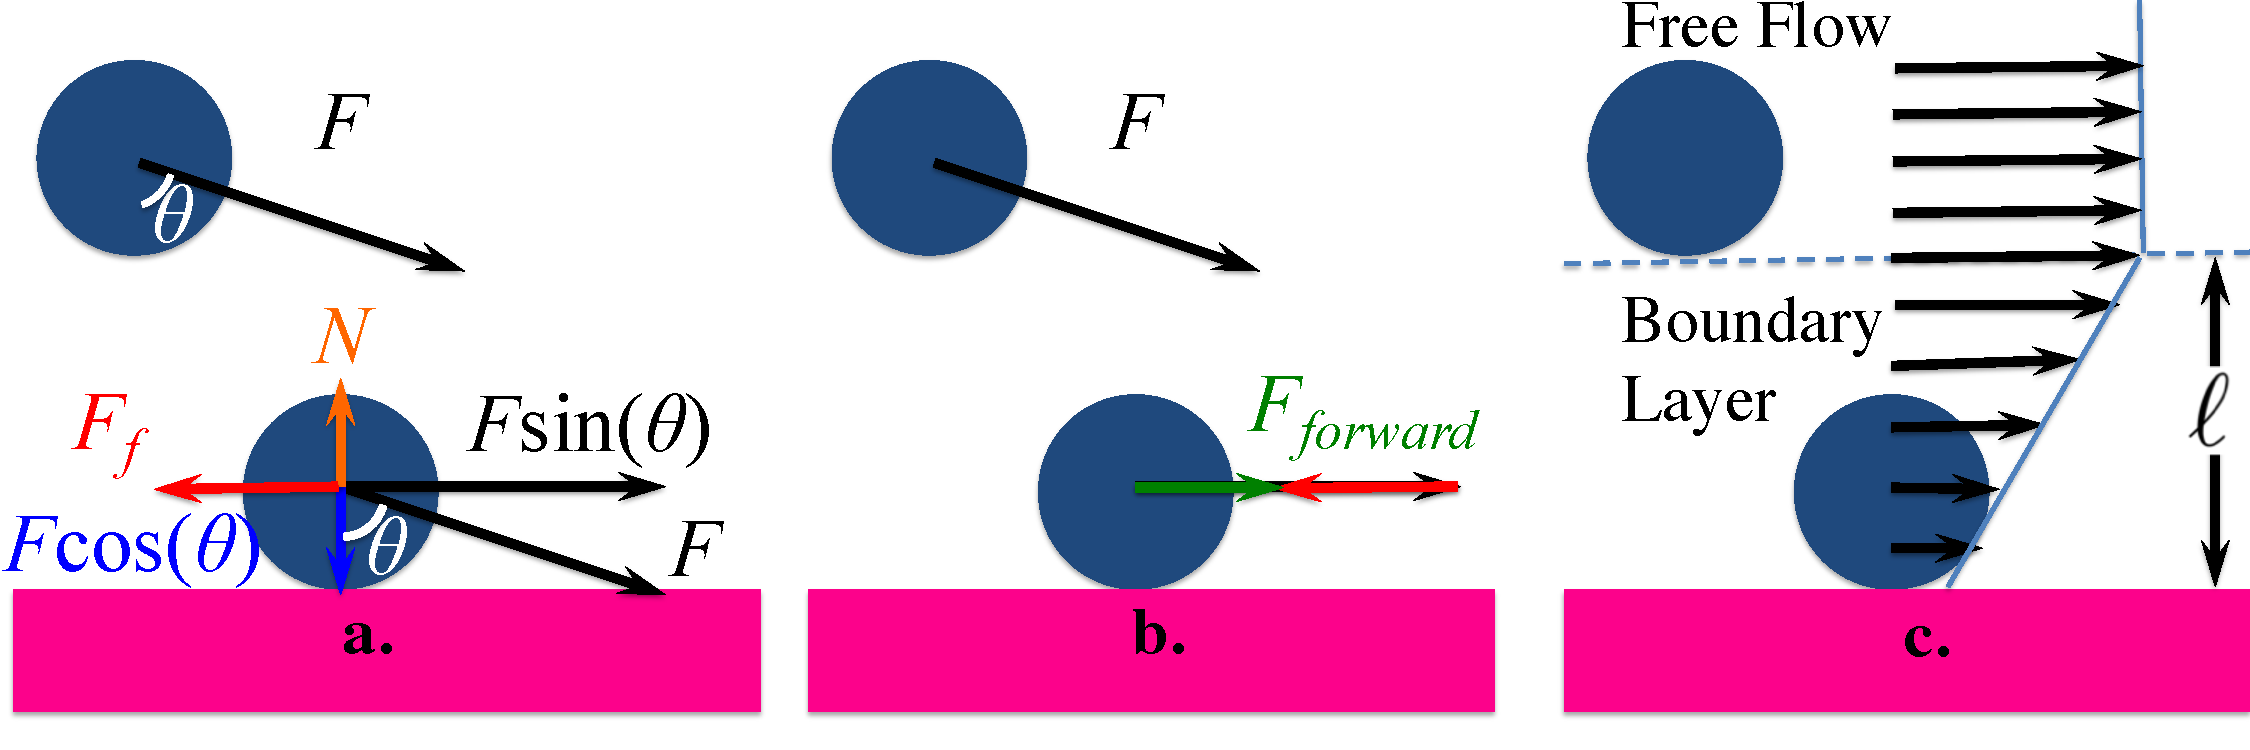
\includegraphics[width=0.8\columnwidth]{friction.pdf} 
\vspace{-1em}
\caption{(a,b) Wall friction reduces the force for going forward $F_{\text{\emph{forward}}}$ on a robot near a wall, but not for a free robot. (c) velocity of a fluid reduces to zero at the boundary.
\label{fig:friction}
}
\end{center}
\end{figure} 



\section{Algorithms}\label{sec:algorithms}
\subsection{Position Control of $2$ Robots Using Wall Friction}\label{sec:PostionControl2Robots}
\begin{figure*}
\centering
\renewcommand{\figwid}{0.4\columnwidth}
{\begin{overpic}[width =\figwid]{S1_1.png}\put(10,15){$t$ = 0 s}
\end{overpic}
\begin{overpic}[width =\figwid]{S1_2.png}\put(10,15){$t$ = 0.14 s}
\end{overpic}
\begin{overpic}[width =\figwid]{S1_3.png}\put(10,15){$t$  = 0.29 s}
\end{overpic}
\begin{overpic}[width =\figwid]{S1_4.png}\put(10,15){$t$  = 0.43 s}
\end{overpic}
\begin{overpic}[width =\figwid]{S1_5.png}\put(10,15){$t$  = 0.76 s}
\end{overpic}}\\
%{\begin{overpic}[width =\figwid]{two_1.jpg}\put(45,75){$t$  = 0 s}
%\end{overpic}
%\begin{overpic}[width =\figwid]{two_2.jpg}\put(45,75){$t$  = 0.25 s}
%\end{overpic}
%\begin{overpic}[width =\figwid]{two_3.jpg}\put(45,75){$t$  = 0.5 s}
%\end{overpic}
%\begin{overpic}[width =\figwid]{two_4.jpg}\put(45,75){$t$  = 0.75 s}
%\end{overpic}
%\begin{overpic}[width =\figwid]{two_5.jpg}\put(45,75){$t$  = 1 s}
%\end{overpic}}\\
%\vspace{.5em}
%{\begin{overpic}[width =\figwid]{S3_1.jpg}\put(45,75){$t$ = 0 s}
%\end{overpic}
%\begin{overpic}[width =\figwid]{S3_2.jpg}\put(45,75){$t$ = 0.25 s}
%\end{overpic}
%\begin{overpic}[width =\figwid]{S3_3.jpg}\put(45,75){$t$  = 0.5 s}
%\end{overpic}
%\begin{overpic}[width =\figwid]{S3_4.jpg}\put(45,75){$t$  = 0.75 s}
%\end{overpic}
%\begin{overpic}[width =\figwid]{S3_5.jpg}\put(45,75){$t$  = 1 s}
%\end{overpic}}
%\vspace{-1em}
\caption{\label{fig:shapeControlMathematica1}{Frames from an implementation of Alg.\ \ref{alg:PosControl2Robots}: two robot positioning using walls with infinite friction. The algorithm only requires friction along the bottom and right walls.
Robot initial positions are shown by a crosshair, and final positions by a circled crosshair.  Dashed lines show the shortest route if robots could be controlled independently.  Solid arrows show path given by  Alg.\ \ref{alg:PosControl2Robots}.
Online demonstration and source code at \citep{Shahrokhi2015mathematicaParticle}.
%The bottom row shows an extreme case where the robots must switch position.
}
%\vspace{-2em}
}
\end{figure*}

Alg.~\ref{alg:PosControl2Robots} uses wall-friction to arbitrarily position two robots in a rectangular workspace.  This algorithm  introduces concepts that will be used for multi-robot positioning. It only requires collisions with two orthogonal walls, in this case, the bottom and left walls. Fig.~\ref{fig:shapeControlMathematica1} shows a Mathematica implementation of the algorithm, and is useful as a visual reference for the following description.

Assume two robots are initialized at $s_1$ and $s_2$ with corresponding goal destinations $e_1$ and $e_2$. 
Denote the current positions of the robots  $r_1$ and $r_2$. 
Subscripts $_x$ and $_y$ denote the $x$ and $y$ coordinates, i.e., $s_{1x}$ and $s_{1y}$ denote the $x$ and $y$ locations of $s_1$. 
The algorithm assigns a global control input at every instance.
The goal is to adjust 
 $\Delta r_x = r_{2x}-r_{1x}$ from $\Delta s_x = s_{2x}-s_{1x}$ to $\Delta e_x = e_{2x}-e_{1x}$ and  adjust 
 $\Delta r_y = r_{2y}-r_{1y}$ from $\Delta s_y = s_{2y}-s_{1y}$ to $\Delta e_y = e_{2y}-e_{1y}$ using a shared global control input. 
 This algorithm exploits the position-dependent friction model \eqref{eq:frictionmodel}.
 %employing the assumption we have made earlier about the walls' friction. 

Our algorithm solves the positioning problem in three steps: 
First, $|\Delta r_x - \Delta e_x |$ is reduced to zero while  $\Delta r_y$ is kept constant in Alg.~\ref{alg:XControl}. 
Second, $|\Delta r_y - \Delta e_y |$ is reduced to zero while  $\Delta r_x$ is kept constant. % in Alg.~\ref{alg:YControl}. 
Third, the robots, now correctly positioned relative to each other, are moved to their goal locations.

In the worse case, adjusting both $\Delta r_x$ and $\Delta r_y$ requires two iterations.   Two iterations of Alg. \ref{alg:XControl} are only required if $|\Delta e_x - \Delta s_x|>L$. 
Similarly,  two iterations %of Alg. \ref{alg:YControl} 
are only required if $|\Delta e_y - \Delta s_y|>L$.  The worst case path length is 6$L$.

%Step (i): Fixing $\Delta r_x$
%\label{theory:step1}
%\begin{enumerate}
%\item
%If $\Delta e_x$ is negative, the robots will be commanded to move toward the left wall and halt $\epsilon$ distance from the left wall.
%If $\Delta e_x \ge 0$, the robots will be commanded to move toward the right wall and halt $\epsilon$ distance from the right wall. The epsilon distance prevents the robots from experiencing friction along the vertical wall.
%\item  let $y_{\min} = \min_i r_{iy}$, i.e., $y_{\min}$ be the minimum height of the two robots. Move both robots downward  $y_{\min}$ such that one of the robots touches the bottom wall and hence friction force will prevent this robot from moving left or right.
%\item friction force holds the lower robot in place while the upper robot may move right and left freely to change $\Delta r_x $ to $\Delta e_x$.
%\item  If after the free move of the upper robot $\Delta r_x$ is not $\Delta e_x$, Step (i) will be repeated.  No more than two iterations of step (i) are required.
%\end{enumerate}
%
%Step (ii): Fixing $\Delta r_y$
%Now that $\Delta r_x$ is corrected, $\Delta r_y$ must be corrected:
%\begin{enumerate}
%\item 
%If $\Delta e_y$ is negative, the robots will be commanded to move toward the top wall and halt $\epsilon$ distance from the top wall.
%If $\Delta e_y \ge 0$, the robots will be commanded to move toward the bottom wall and halt $\epsilon$ distance from the bottom wall. The epsilon distance prevents the robots from experiencing friction along the horizontal wall.
%\item  let $x_{\min} = \min_i r_{ix}$, i.e., $x_{\min}$ be the minimum distance of the two robots from the origin along the $x$-axis. Move both robots to the left $x_{\min}$ such that one of the robots  touches the left wall and hence friction force will prevent this robot from moving up or down.
%\item  friction force holds the left robot in place while the right robot may move up or down freely to change $\Delta r_y $  to $\Delta e_y$.
%\item  If after the free move of the right robot $\Delta r_y$ is not $\Delta e_y$, Step (ii) will be repeated.  No more than two iterations of step (ii) are required.
%\end{enumerate}
%Once $\Delta r_x$ and $\Delta r_y$ are set to $\Delta e_x$ and $\Delta e_y$, a straight-line global input moves both robots from $r_1$ and $r_2$ to $e_1$ and $e_2$. 
%

\begin{algorithm}
\caption{WallFrictionArrange2Robots($s_1,s_2,e_1,e_2,L$)}\label{alg:PosControl2Robots}
\begin{algorithmic}[1]
\Require starting $(s_1,s_2)$ and ending $(e_1,e_2)$ positions of  two robots. 
$(0,0)$ is bottom corner, $s_1$ is rightmost robot, 
 $L$ is length of the walls. 
 Current robot positions are $(r_1,r_2)$.

\State  GenerateDesired$x$-spacing($s_1,s_2,e_1,e_2,L$)
\State  GenerateDesired$y$-spacing($r_1,r_2,e_1,e_2,L$)
\State Move robots $e_1 - r_1$

\end{algorithmic}
\end{algorithm}


\begin{algorithm}
\caption{GenerateDesired$x$-spacing($s_1,s_2,e_1,e_2,L$)}\label{alg:XControl}
\begin{algorithmic}[1]
\Require knowledge of starting $(s_1,s_2)$ and ending $(e_1,e_2)$ positions of  two robots. 
$(0,0)$ is bottom corner, $s_1$ is topmost robot, 
 $L$ is length of the walls. Current robot positions are $(r_1,r_2)$.
\Ensure   $ r_{1y} - r_{2y}  \equiv s_{1y} - s_{2y} $   %$\Delta y(t) \equiv \Delta y(0)$ 
\State $\epsilon \gets $ small number
\State $ \Delta s_x  \gets s_{1x} - s_{2x} $
\State $ \Delta e_x \gets e_{1x} - e_{2x} $
%\State $ r_1 \gets s_1$, $ r_2 \gets s_2$
\If {$\Delta e_x < 0 $ }
\State move$( L-\epsilon-\max( r_{1x},r_{2x}) ,0)   $ \Comment{To right wall}
\Else 
\State  move$ ( \epsilon-\min( r_{1x},r_{2x}),0 )    $ \Comment{Move to left wall}
\EndIf
\State move$(0, -\min( r_{1y},r_{2y} ))$ \Comment{Move to bottom}
%\State $ r_1 \gets r_1+m$, $ r_2 \gets r_2+m$ \Comment{Apply move}
\If {$\Delta e_x - (r_{1x} - r_{2x} ) > 0 $}
\State move$(\min(|\Delta e_x - \Delta s_x |, L- r_{1x}), 0)$  \Comment{Move right}
\Else
\State move$(-\min(|\Delta e_x - \Delta s_x |, r_{1x}), 0)$\Comment{Move left}
\EndIf 
\State move$(0, \epsilon)$ \Comment{Move up}
%\State $ r_1 \gets r_1+m$, $ r_2 \gets r_2+m$ \Comment{Apply move}
%\State $\Delta r_x = r_{1x} - r_{2x}$
\If {$r_{1x} - r_{2x} \equiv \Delta e_x$} 
%\State   $ m \gets (e_{1x}-r_{1x}, e_{1y}-r_{1y})$
%\State $ r_1 \gets r_1+m$, $ r_2 \gets r_2+m$ \Comment{Apply move}
\State  \Return $(r_1,r_2)$
\Else   
\State \Return GenerateDesired$x$-spacing($r_1,r_2,e_1,e_2,L$)
\EndIf
\end{algorithmic}
\end{algorithm}

%\begin{algorithm}
%\caption{GenerateDesired$y$-spacing($s_1,s_2,e_1,e_2,L$)}\label{alg:YControl}
%\begin{algorithmic}[1]
%\Require Knowledge of starting $(s_1,s_2)$ and ending $(e_1,e_2)$ positions of  two robots. 
%$(0,0)$ is bottom corner, $s_1$ is rightmost robot, 
% $L$ is length of the walls. Current robot positions are $(r_1,r_2)$.
%\Ensure   $ r_{1x} - r_{2x}  \equiv s_{1x} - s_{2x} $   %$\Delta y(t) \equiv \Delta y(0)$ 
%\State $ \Delta s_y  \gets s_{1y} - s_{2y} $
%\State $ \Delta e_y \gets e_{1y} - e_{2y} $
%\State $ r_1 \gets s_1$, $ r_2 \gets s_2$
%\If {$\Delta e_y < 0 $ }
%\State $ m \gets ( L-\max( r_{1y},r_{2y}) ,0)   $ \Comment{Move to top wall}
%\Else 
%\State  $ m \gets ( -\min( r_{1y},r_{2y}),0 )    $ \Comment{Move to bottom wall}
%\EndIf
%\State $m  \gets  m + (0, -\min( r_{1x},r_{2x} ))$ \Comment{Move to left}
%\State $ r_1 \gets r_1+m$, $ r_2 \gets r_2+m$ \Comment{Apply move}
%\If {$\Delta e_y - (r_{1y} - r_{2y} ) > 0 $}
%\State $ m \gets (\min(|\Delta e_y - \Delta s_y |, L- r_{1y}), 0)$  \Comment{Move top}
%\Else
%\State $ m \gets (-\min(|\Delta e_y - \Delta s_y |, r_{1y}), 0)$\Comment{Move bottom}
%\EndIf 
%\State $m  \gets  m + (0, \epsilon)$ \Comment{Move right}
%\State $ r_1 \gets r_1+m$, $ r_2 \gets r_2+m$ \Comment{Apply move}
%\State $\Delta r_y = r_{1y} - r_{2y}$
%\If {$\Delta r_y \equiv \Delta e_y$} 
%\State   $ m \gets (e_{1x}-r_{1x}, e_{1y}-r_{1y})$
%\State $ r_1 \gets r_1+m$, $ r_2 \gets r_2+m$ \Comment{Apply move}
%\State  \Return $(r_1,r_2)$
%\Else   
%\State \Return GenerateDesired$y$-spacing($r_1,r_2,e_1,e_2,L$)
%\EndIf
%\end{algorithmic}
%\end{algorithm}






\subsection{Position Control of $n$ Robots Using Wall Friction}\label{sec:PostionControlnRobots}
Alg. \ref{alg:PosControl2Robots}  can be extended to control the position of $n$ robots using wall friction under several constraints. The solution described here is an iterative procedure with $n$ loops. The $k$th loop moves the $k$th robot from a \emph{staging zone} to the desired position in a \emph{build zone}. All robots move according to the global input, but due to wall friction, at the end the $k$th loop, robots 1 through $k$ are in their desired final configuration in the build zone, and robots $k+1$ to $n$ are in the staging zone. See Fig.~\ref{fig:construction2d} for a schematic of the build and staging zones.


\begin{figure}
\begin{center}
	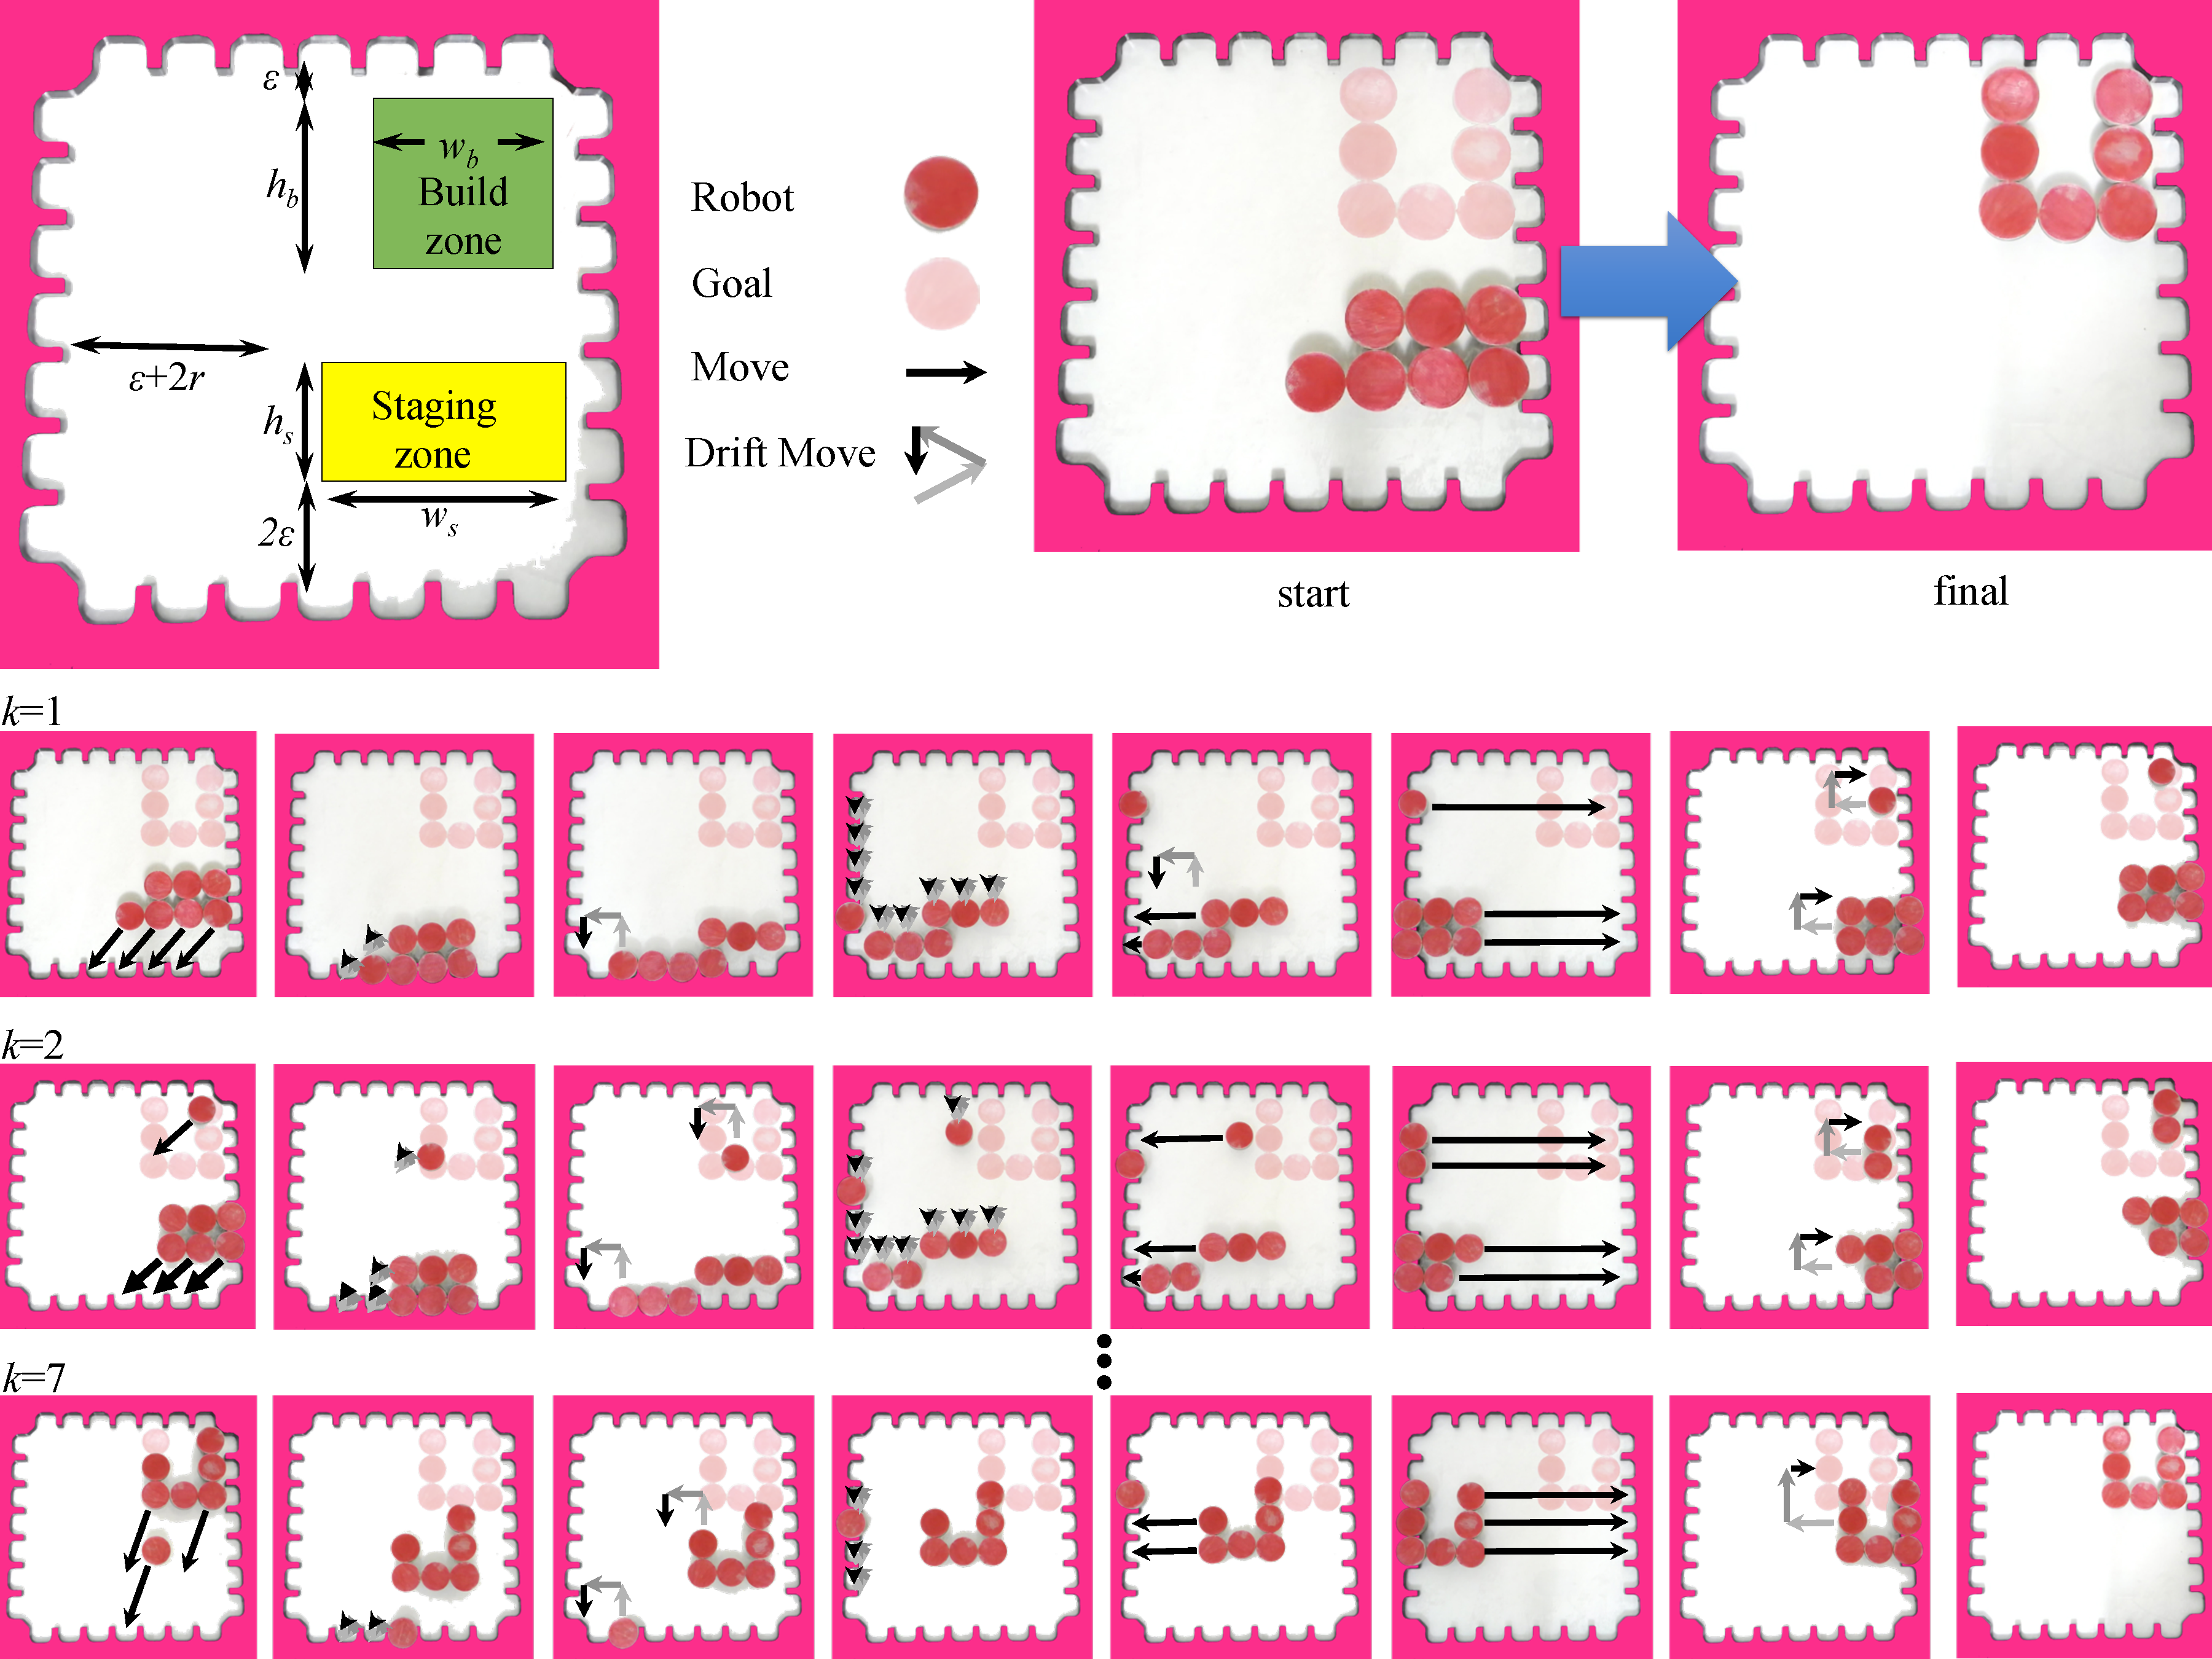
\includegraphics[width=1.0\columnwidth]{multirobotSliderHardware.pdf}
\end{center}
\vspace{-1em}
\caption{\label{fig:construction2d}
Illustration of Alg.\ \ref{alg:PosControlNRobots}, $n$ robot position control  using wall friction.
}
\end{figure}


Assume an open workspace with four axis-aligned walls with infinite friction.
The axis-aligned build zone of dimension $(w_b, h_b)$ containing the final configuration of $n$ robots must be disjoint from the axis-aligned staging zone of dimension $(w_s, h_s)$  containing the starting configuration of $n$ robots. Without loss of generality, assume the build zone  is above the staging zone. 
Furthermore, there must be at least $\epsilon$ space above the build zone, $\epsilon$ below the staging zone, and $\epsilon + 2r$ to the left of the build and staging zone, where $r$ is the radius of a robot.  The minimum workspace is then $(\epsilon + 2r + \max(w_b,w_s), 2\epsilon + h_s,h_b)$.

The $n$ robot position control algorithm relies on a $\operatorname{DriftMove}(\alpha, \beta, \epsilon)$ control input, shown in Fig.\  \ref{fig:driftmove}.
A drift move consists of repeating a triangular movement sequence $\{ (\beta/2,-\epsilon),(\beta/2,\epsilon),(-\alpha,0)\}$. The robot touching a top wall moves right $\beta$ units, while robots not touching the top move right $\beta-\alpha$.

\begin{figure}
\begin{center}
	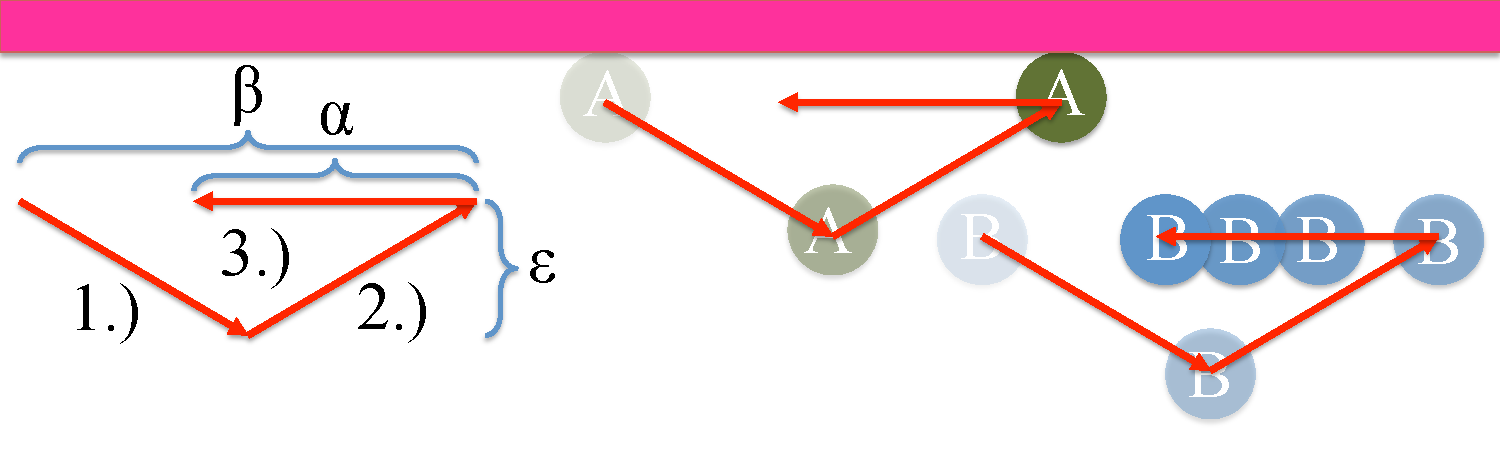
\includegraphics[width=.9\columnwidth]{driftmove.pdf}
\end{center}
\vspace{-1em}
\caption{\label{fig:driftmove}
A  $\operatorname{DriftMove}(\alpha, \beta, \epsilon)$ to the right repeats a triangular movement sequence $\{ (\beta/2,-\epsilon),(\beta/2,\epsilon),(-\alpha,0)\}$. Robot $A$ touching a top wall moves right $\beta$ units, while robots not touching the top move right $\beta-\alpha$.}
\end{figure}

Let $(0,0)$ be the lower left corner of the workspace, $p_k$ the $x,y$ position of the $k$th robot, and $f_k$ the final $x,y$ position of the $k$th robot. Label the robots in the staging zone from left-to-right and bottom-to-top, and the $f_k$ configurations top-to-bottom and right-to-left as shown in Fig.~\ref{fig:construction2d}.

\begin{algorithm}
\caption{PositionControl$n$RobotsUsingWallFriction($k$)}\label{alg:PosControlNRobots}
\begin{algorithmic}[1]
\State move( $-\epsilon, r-p_{ky}$) % move  away from right wall and down till robot k touches bottom


\While{ $p_{kx} > r$} 
\State $\operatorname{DriftMove}(\epsilon, \min(p_{kx} - r,\epsilon), \epsilon)$ left   %drift move left until kth robot touches left wall
\EndWhile

\State $m \gets \operatorname{ceil}(\frac{f_{ky}-r}{\epsilon})$
\State $\beta \gets \frac{f_{ky}-r}{m}$
\State $\alpha \gets \beta - \frac{r - p_{ky}-\epsilon}{m}$
\For{ $m$ iterations}
\State $\operatorname{DriftMove}(\alpha, \beta, \epsilon)$ up   %move kth robot to f_{ky} and leave the rest in position.
\EndFor

\State move($r+\epsilon-f_{kx}, 0$)  % move the group to the left until k is in the correct relative x position
\State move($f_{kx}-r, 0$)  

\end{algorithmic}
\end{algorithm}

Alg. \ref{alg:PosControlNRobots} proceeds as follows:  
First, the robots are moved left away from the right wall, and down so robot $k$ touches the bottom wall.
Second, a set of $\operatorname{DriftMove}$s are executed that move robot $k$ to the left wall with no net movement of the other robots.
Third, a set of $\operatorname{DriftMove}$s are executed that  move robot $k$ to its target height and return the other robots to their initial heights. 
Fourth, all robots except robot $k$ are pushed left until robot $k$ is in the correct relative $x$ position compared to robots 1 to $k-1$.
Finally, all robots are moved right until robot $k$ is in the desired target position. Running time is $O(n(w+h))$.


\subsection{Controlling Covariance Using Wall Friction}\label{subsec:ClosedLoopCovarianceControl}
Assume an open workspace with infinite boundary friction. Goal variances and covariance are  $(\sigma_{goalx}^2,\sigma_{goaly}^2, \sigma_{goalxy})$ and mean, variances and covariance of the swarm  are $( \bar{x},\bar{y},\sigma_x^2,\sigma_y^2, \sigma_{xy})$. 
%$\sigma_x^2$ decreases when the swarm is pushed into vertical walls, and $\sigma_y^2$ decreases when the swarm is pushed into horizontal walls. Alg.~\ref{alg:CovCont} procedes as follows:
\begin{enumerate}
\item swarm pushed into the left wall until $\sigma_x^2 \le c_1\sigma_{goalx}^2$.  
\item swarm's mean position is moved to the center of the workspace
\item swarm pushed into the bottom wall until $\sigma_y^2 \le  \sigma_{goaly}^2$. 
\item if $\sigma_{goalxy}>0$ swarm slides right until $\sigma_{xy} \ge \sigma_{goalxy}$ \\
else swarm slides left until $\sigma_{xy} \le \sigma_{goalxy}$ 
\item  swarm's mean position is moved to the center of the workspace
\end{enumerate}
The constant $c_1$ in step 1 should be less than 1 to ensure $\sigma_x^2$ stays within tolerance during the subsequent moves.


%\begin{algorithm}
%\caption{Swarm Covariance Control With Wall Friction}\label{alg:CovCont}
%\begin{algorithmic}[1]
%\Require  goal variances and covariance and mean, variances and covariance of the swarm  $(\sigma_{goalx}^2,\sigma_{goaly}^2, \sigma_{goalxy}, \bar{x},\bar{y},\sigma_x^2,\sigma_y^2, \sigma_{xy})$. 
%%Swarm is Gaussian distributed (in limit it is uniformly distributed), 
%$L_w$ is width of the walls and $L_h$ is the height of the wall. $(0,0)$ is top right corner. $\epsilon$ is the error for reaching covariance.
%\If {$\sigma_x^2 > \sigma_{goalx}^2/10 $ }
%\State $ \bar{x} \gets \sigma_{goalx}/10   $ \Comment{Move to left wall}
%\State $MoveToCenter \gets true$
%\Else
%\If {$MoveToCenter$ }
%\State   $ \bar{x} \gets L_w/2 $, $\bar{y} \gets L_h/2 $ \Comment{Move to the center}
%\State $MoveToBottom \gets true$
%\State $MoveToCenter \gets false$
%\Else 
%\If {$MoveToBottom $}
%\State $ \bar{y} \gets L_h - \sigma_{goaly}   $ \Comment{Move to bottom}
%\State $MoveToBottom \gets false$
%\Else
%\If {$\sigma_{xy} -\sigma_{goalxy} > \epsilon$}
%\While  {$\sigma_{xy} -\sigma_{goalxy} > \epsilon$ }
%\State $ \bar{x} \gets \bar{x} + \epsilon  $ \Comment{Move to right wall}
%\EndWhile
%\Else
%\If {$\sigma_{xy} -\sigma_{goalxy} < \epsilon$ }
%\While  {$\sigma_{xy} -\sigma_{goalxy} < \epsilon$ }
%\State $ \bar{x} \gets \bar{x} - \epsilon  $ \Comment{Move to left wall}
%\EndWhile
%\EndIf
%\EndIf
%\EndIf
%\EndIf
%\EndIf
%\State   $ \bar{x} \gets L_w/2 $, $\bar{y} \gets L_h/2 $ \Comment{Move to the center}
%
%\end{algorithmic}
%\end{algorithm}







